\documentclass{beamer}
\usepackage[utf8]{inputenc}
\usepackage{amsmath, amssymb, amsfonts, amsthm, mathtools,mathrsfs, commath}
%\usepackage[inline]{enumitem}
\usepackage{parskip}
\usepackage{physics}
\usepackage{amsmath}
\usepackage{tikz}
\usepackage{mathdots}
\usepackage{yhmath}
\usepackage{cancel}
\usepackage{color}
\usepackage{siunitx}
\usepackage{array}
\usepackage{multirow}
\usepackage{amssymb}
\usepackage{gensymb}
\usepackage{tabularx}
\usepackage{extarrows}
\usepackage{booktabs}
\usetikzlibrary{fadings}
\usetikzlibrary{patterns}
\usetikzlibrary{shadows.blur}
\usetikzlibrary{shapes}



\usetheme{Madrid}
\useoutertheme{infolines}
\usecolortheme{default}


\newcommand{\R}{\mathbb{R}}
\newcommand{\vphi}{\varphi}
%------------------------------------------------------------
%This block of code defines the information to appear in the
%Title page
\title[MA 556 Presentation] %optional
{MA 556: Differential Geometry}

\subtitle{Group 2 Presentation}

\author[Sanjyot Shenoy] % (optional)
{Sanjyot Shenoy}

\institute[IIT-B] % (optional)
{
  18B030023 \\
  Indian Institute of Technology, Bombay
}

\date[2/9/2021] % (optional)
{2/9/2021}

%\logo{\includegraphics[height=1cm]{overleaf-logo}}

%End of title page configuration block
%------------------------------------------------------------



%------------------------------------------------------------
%The next block of commands puts the table of contents at the 
%beginning of each section and highlights the current section:

\AtBeginSection[]
{
  \begin{frame}
    \frametitle{Speakers}
    \tableofcontents[ 
    currentsection
    ] 
  \end{frame}
}
%------------------------------------------------------------


\begin{document}

%The next statement creates the title page.
\frame{\titlepage}


%---------------------------------------------------------
%This block of code is for the table of contents after
%the title page
\begin{frame}
\frametitle{Table of Contents}
\tableofcontents[]
\end{frame}
%---------------------------------------------------------



%---------------------------------------------------------
\section{Question 3, from Topological Manifolds Section}
\begin{frame}{Question 1}
\begin{block}{Question 3, from Topological Manifolds Section}
Show that a topological space $\displaystyle X$ is locally $n$-euclidean iff$\displaystyle ( \Leftrightarrow )$ every point $\displaystyle x\in X$ has a neighborhood homeomorphic to an open set of $\displaystyle \mathbb{R}^{n}$.
\end{block}
\end{frame}

\begin{frame}{Prerequisites for Question 1}
Let us recall the concepts required for this question.
\begin{block}{Locally $\displaystyle n$-euclidean}
A topological space $\displaystyle X$ is \alert{locally $n$-euclidean} if every point of $\displaystyle X$ has a neighborhood homeomorphic to $\displaystyle \mathbb{R}^{n}$ for some $\displaystyle n$.
Equivalently $\displaystyle X$ is locally euclidean iff every point of $\displaystyle X$ has a neighborhood homeomorphic to an open $\displaystyle n$-ball for some $\displaystyle n$.
\end{block} 
where open $\displaystyle n$-ball of radius $\displaystyle r$ around $\displaystyle x_{0} \in \mathbb{R}^{n}$ is $\displaystyle B^{n}( x_{0} ,r) =\left\{x\in \mathbb{R}^{n} \ |\ ||x_{0} -x||< r\right\}$ 
\begin{block}{Homeomorphism}
Let $\displaystyle X,Y$ be two topological spaces. A bijective map $\displaystyle f:X\rightarrow Y$ is said to be a \alert{homeomorphism} if $\displaystyle f$ and $\displaystyle f^{-1}$ are continuous. 
\end{block}
\end{frame}
\begin{frame}{Prerequisites for Question 1 (contd.)}
\begin{block}{Open Set in Metric Topology}
A subset $\displaystyle U$ of a metric space $\displaystyle X$ is open (in the metric topology) if $\displaystyle \forall x\in U$, there exists a $\displaystyle r >0$ such that $\displaystyle B( x,r) \subseteq U$.
\end{block}
\end{frame}
\begin{frame}{Sketch of Proof}
We have a two-way traffic ($\displaystyle \Leftrightarrow $) here. 

First we note that, the $\displaystyle \Rightarrow $ direction follows from definition of locally $\displaystyle n$-euclidean spaces. 

\alert{The trouble lies in proving the converse!}
\end{frame}
\begin{frame}{Sketch of Proof (contd.)}
Now, for the converse ($\displaystyle \Leftarrow $) part,

For each point \ $\displaystyle x\in X$ \ we have a neighborhood, $\displaystyle V_{x}$ say, homeomorphic to an open set, let's say $\displaystyle U_{x}$ of $\displaystyle \mathbb{R}^{n}$. 

From this information, we need to construct a homeomorphism from an open neigbourhood of $\displaystyle x$ to either $\displaystyle \mathbb{R}^{n}$ or an open $\displaystyle n$-ball 

How to go about this? 

We will use two facts 
\begin{enumerate}
\item open $\displaystyle n$-balls form a basis for topology on $\displaystyle \mathbb{R}^{n}$, and hence are open, 
\item definition of an open set in a metric space 
\end{enumerate}

Then restrict ourselves to an open $\displaystyle n$-ball inside the open set, then trace it back to its domain in $\displaystyle X$ 
\end{frame}
\begin{frame}{Diagram}
\begin{figure}
    \centering
    \centering
    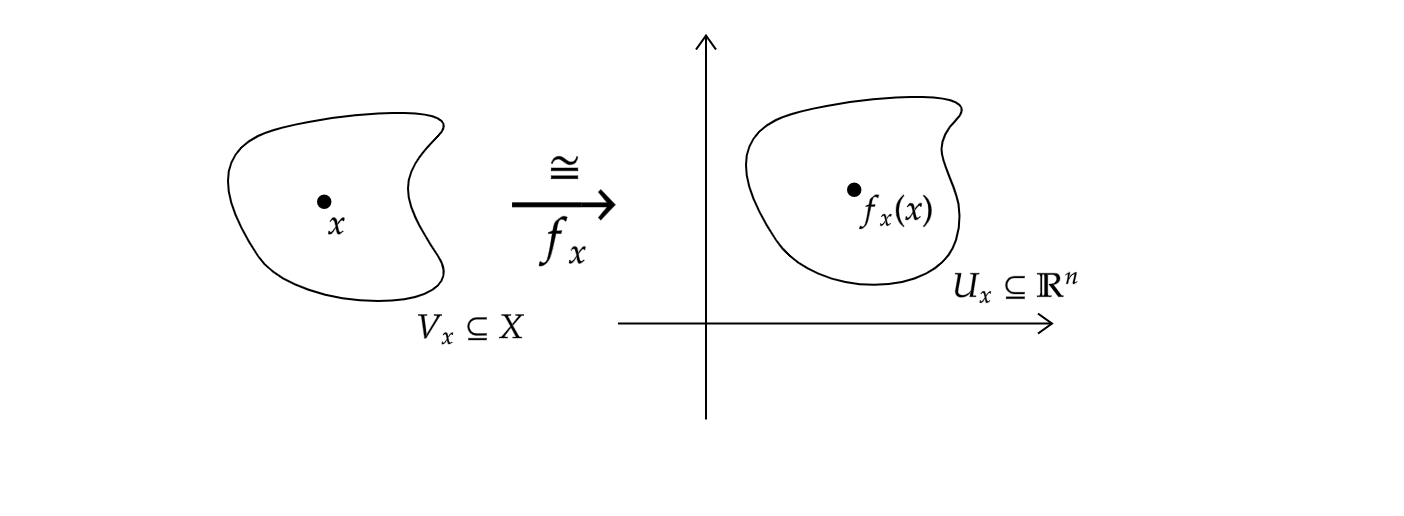
\includegraphics[width = 1.1\textwidth]{diag-1.png}

    %\includegraphics{}
    %\label{fig:my_label}
\end{figure}
Note here the subscripts represent that the functions and the sets \alert{depend} on $x$.
\end{frame}
\begin{frame}{Proof of Question 1}
Now we get to the explicit details. 
\begin{block}{Proof}
($\displaystyle \Rightarrow $): Here $\displaystyle X$ is locally $\displaystyle n$-euclidean, hence, by our criterion, for each $\displaystyle x\in X$, we have a neighbourhood homeomorphic to $\displaystyle \mathbb{R}^{n}$. Since $\displaystyle \mathbb{R}^{n}$ is an open set in $\displaystyle \mathbb{R}^{n}$, we are done. 

Equivalently, $\displaystyle X$ is locally $\displaystyle n$-euclidean, hence, for each $\displaystyle x\in X$, we have a neighbourhood homeomorphic to an open $\displaystyle n$-ball, and since open $\displaystyle n$-balls are open sets in \ $\displaystyle \mathbb{R}^{n}$, we are done. 
\end{block}
\end{frame}
\begin{frame}
\begin{block}{Proof(contd.)}
($\displaystyle \Leftarrow $): Let us suppose that for each $\displaystyle x\in X$, we have a neighborhood $\displaystyle V_{x}$ \ homeomorphic to an open set $\displaystyle U_{x} \subseteq \mathbb{R}^{n}$, via the homeomorphism $\displaystyle f_{x}$.  

Since $\displaystyle U_{x}$ is an open set in $\displaystyle \mathbb{R}^{n}$, which is a metric space, and we have $\displaystyle f_{x}( x) \in U_{x}$, then, there exists an open $\displaystyle n$-ball $\displaystyle B( f_{x}( x) ,r)$ such that $\displaystyle B( f_{x}( x) ,r) \subseteq U_{x}$. 


Since $\displaystyle f_{x}$ is a homeomorphism $\displaystyle \Rightarrow $ $\displaystyle f_{x}^{-1}( B( f_{x}( x) ,r))$ is an open set in $\displaystyle X$. Let $\displaystyle V'_{x} =f_{x}^{-1}( B( f_{x}(x),r))$. Clearly, $\displaystyle x\in V'_{x}$, since $\displaystyle f_{x}( x) \in B( f_{x}(x),r)$. Thus $\displaystyle V'_{x}$ is a neighbourhood of $\displaystyle x$. 

Consider the restriction, $\displaystyle h_{x}$ of $\displaystyle f_{x}$ to $\displaystyle V'_{x}$, that is $\displaystyle h_{x} =f_{x} |_{V'_{x}} :\ V'_{x}\rightarrow B( f_{x}( x) ,r)$, then

\textbf{Claim}: $\displaystyle h_{x}$ is a homeomorphism. 

\textbf{Proof of Claim}: Since $\displaystyle f_{x}$ is bijective on $\displaystyle V_{x}$, it in injective on $\displaystyle V'_{x}$, surjectivity follows since$\displaystyle V'_{x} =f_{x}^{-1}( B( x,r))$. Continuity of $\displaystyle h_{x}$ follows from continuity of $\displaystyle f_{x}$ and similarly for $\displaystyle h_{x}^{-1}$. 

Hence for each $\displaystyle x\in X$, we have a neigbourhood which is homeomorphic to an open $\displaystyle n$-ball, hence, $\displaystyle X$ is locally $\displaystyle n$-euclidean. $\displaystyle \qed $ 
\end{block}
\end{frame}
\begin{frame}{Diagram}
\begin{figure}
    \centering
    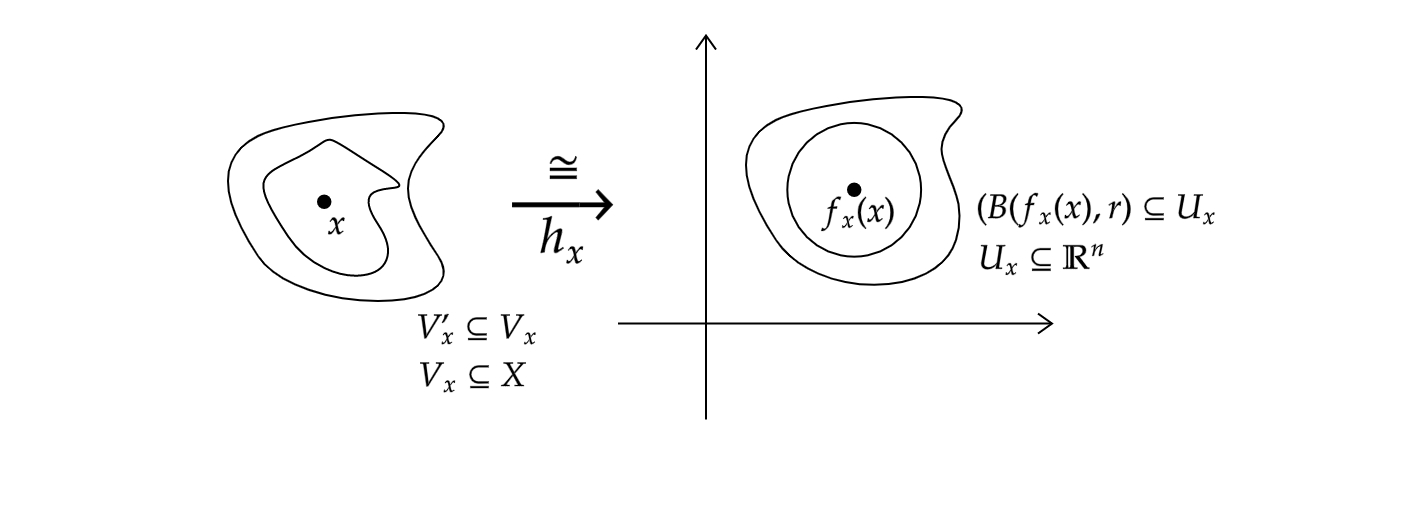
\includegraphics[width = 1.1\textwidth]{diag-2.png}
    \caption{A pictorial view of the construction}
\end{figure}
\end{frame}


\section{Question 4, from Topological Manifolds Section}
\begin{frame}{Question 2}
\begin{block}{Question 4, from Topological Manifolds Section}
Consider the three conditions on a topological space in the definition of a topological manifold. Think of examples which satisfy two of those conditions
but not the third.
\end{block}
\end{frame}

\begin{frame}{Prerequisites for Question 2}
Let $X$ be a topological space.
\begin{block}{Second Countable}
$\displaystyle X$ is \alert{second countable} if it has a countable basis. 
\end{block}
\begin{block}{Locally $n$-euclidean}
A topological space $\displaystyle X$ is \alert{locally $n$-euclidean} if every point of $\displaystyle X$ has a neighborhood homeomorphic to $\displaystyle \mathbb{R}^{n}$ for some $\displaystyle n$.


Equivalently $\displaystyle X$ is locally
euclidean iff every point of $\displaystyle X$ has a neighborhood homeomorphic to an open $\displaystyle n$-ball for some $\displaystyle n$.


\end{block}
\begin{block}{Hausdorff Space}
$\displaystyle X$ is \alert{Hausdorff} if for any distinct points $\displaystyle x,y\in X$, there exist neighborhoods of $\displaystyle x$ and $\displaystyle y$ which are disjoint.
\end{block}
\end{frame}
\begin{frame}{Prerequisites for Question 2 (contd.)}
\begin{block}{Topological Manifold}
$\displaystyle X$ is a topological manifold if it is Hausdorff, second countable, and locally $\displaystyle n$-euclidean for some $\displaystyle n$.
\end{block}
\end{frame}
\begin{frame}{Solution to Question 2}
\begin{exampleblock}{Example 1: Hausdorff and Second Countable but not locally euclidean}
$\displaystyle X=[ 0,1] \subseteq \mathbb{R}$, with the subspace topology. Then, $\displaystyle X$ is Hausdorff, since $\displaystyle \mathbb{R}$ is Hausdorff. It is also second coutable since $\displaystyle \mathbb{R}$ is. 

However it is not locally euclidean! 

To see this, note that, $\displaystyle ( 0,1) \subseteq \mathbb{R}$ under subspace topology is locally $\displaystyle 1$-euclidean, hence we will try to see if $\displaystyle X$ is locally $\displaystyle n$-euclidean, for $\displaystyle n=1$, $\displaystyle n >1$ is not possible, since if it is, then $\displaystyle ( 0,1)$ will also be $\displaystyle n$-euclidean for this $\displaystyle n$, which is not possible, as $\displaystyle ( 0,1) =B\left(\frac{1}{2} ,\frac{1}{2}\right)$, which cannot be homeomorphic to any open set in $\displaystyle \mathbb{R}^{n}$ as a consequence of invariance of domain theorem of Brouwer.

\end{exampleblock}
\end{frame}
\begin{frame}{Solution to Question 2 (contd.)}
\begin{exampleblock}{Example 1(contd.)}
Suppose, $\displaystyle X$ is locally $\displaystyle 1$-euclidean, then every for every point in $\displaystyle X$, it has a neighbourhood which is homeomorphic to a $\displaystyle 1$-ball, which is a an interval in $\displaystyle \mathbb{R}$. 

Then, this should hold for $\displaystyle 0$ and $\displaystyle 1$ as well. Note that open neigbourhoods of $\displaystyle 0$ and $\displaystyle 1$ in $\displaystyle X$ look like $\displaystyle [ 0,a)$ and $\displaystyle ( b,1]$, where $\displaystyle a,b\in ( 0,1)$, respectively, which are half intervals. Half intervals are not homeomorphic to open intervals, and thus $\displaystyle X$ is not locally $\displaystyle 1$-euclidean, and not thus not locally euclidean. 
\end{exampleblock}  
\end{frame}
\begin{frame}{Solution to Question 2 (contd.)}
\begin{alertblock}{Example 2: Locally Euclidean and Second Countable but not Hausdorff}
One of such examples is the real line with two origins. 

Explicitly,

It is the quotient space of two copies of real line, obtained by identifying any two points with same $\displaystyle x$-coordinate, that is 
\begin{equation*}
\mathbb{R} \times \{a\}\text{ and }\mathbb{R} \times \{b\}
\end{equation*}
with equivalence relation defined by 
\begin{equation*}
( x,a) \sim ( x,b) ,\ \text{if} \ x\neq 0
\end{equation*}
Pictorially this looks like:
\end{alertblock}  
\end{frame}


\begin{frame}{Solution to Question 2 (contd.)}
\begin{alertblock}{Example 2(contd.)}
\begin{figure}
    \centering
    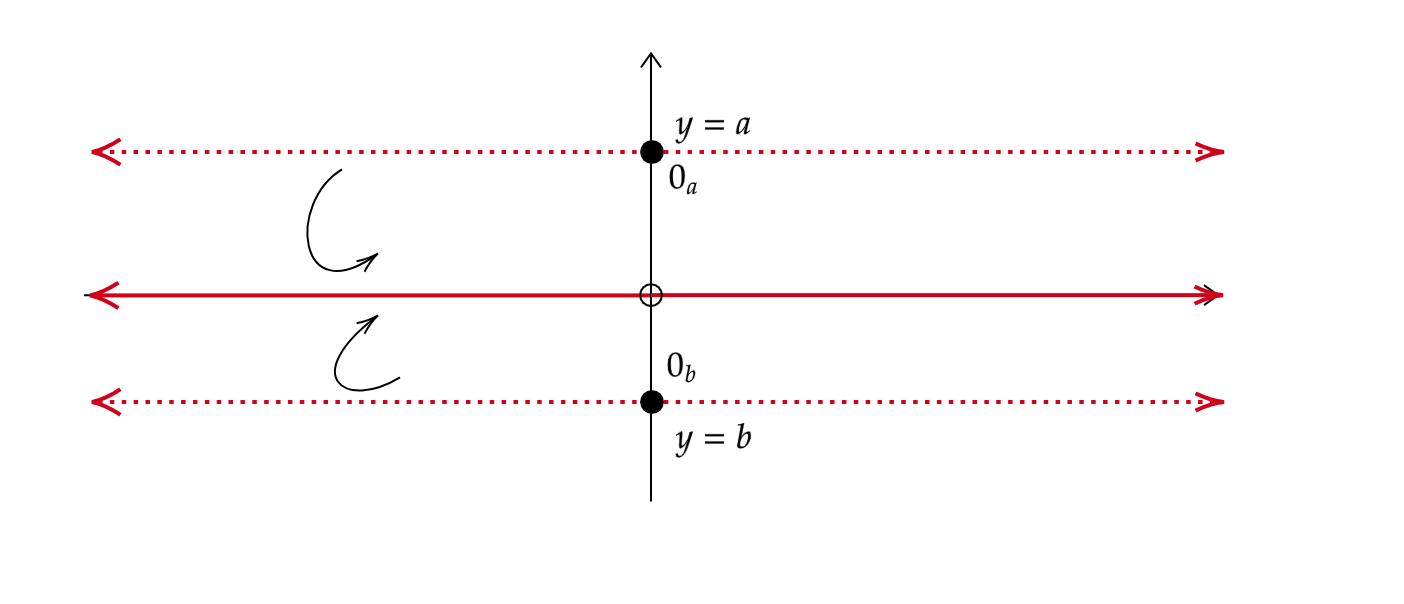
\includegraphics[width = 1.1\textwidth]{diag-3.png}
    \caption{A pictorial view of the construction}
\end{figure}

\end{alertblock}  
\end{frame}

\begin{frame}{Solution to Question 2 (contd.)}
\begin{alertblock}{Example 2(contd.)}
Thus, we have that, for $\displaystyle x=0$, two points, denoted by $\displaystyle 0_{a}$ and $\displaystyle 0_{b}$. Any neigbourhood of $\displaystyle 0_{a}$ looks like  

$\displaystyle B( 0_{a} ,\epsilon ) =\{r\in \mathbb{R} \backslash \{0\} |-\epsilon < r< \epsilon \} \ $and similarly for $\displaystyle 0_{b}$. Thus, all neighbourhoods intersect, and thus these points cannot be separated, and hence this space is not Hausdorff. 

Second countability and locally $\displaystyle 1$-euclidean property follows from respective properties of $\displaystyle \mathbb{R}$ 
\end{alertblock}  
\end{frame}


\begin{frame}{Solution to Question 2 (contd.)}
\begin{block}{Example 3: Hausdorff and Locally Euclidean, but not second countable.}
Form $\displaystyle X=\mathbb{R} \times \mathbb{R}_{d}$, that is product topology of $\displaystyle \mathbb{R}$ with it's standard topology and $\displaystyle \mathbb{R}$ with it's discrete topology.

It is a topological space under the product topology, it is Hausdorff since both $\displaystyle \mathbb{R}$ and $\displaystyle \mathbb{R}_{d}$ are Hausdorff Spaces.

The discrete topology on $\displaystyle \mathbb{R}$ can be given by the following metric: 
\begin{gather*}
d( x,y) =1,\ x\neq y\\
d( x,y) =0,\ x=y
\end{gather*} 
Thus the only possible balls around a point $\displaystyle x\in \mathbb{R}$ are $\displaystyle \mathbb{R}$ or $\displaystyle \{x\}$, which implies that, $\displaystyle \mathbb{R}_{d}$ is $\displaystyle 0$-euclidean.

It is locally euclidean, since $\displaystyle \mathbb{R}$ is locally euclidean, and so is $\displaystyle \mathbb{R}_{d}$ is locally euclidean. 

However it is not second-countable since $\displaystyle \mathbb{R}_{d}$ is not second countable. 
Pictorially, this looks like:
\end{block}  
\end{frame}

\begin{frame}{Diagram for Example 3}
\begin{block}{Example 3(contd.)}
\begin{figure}
    \centering
    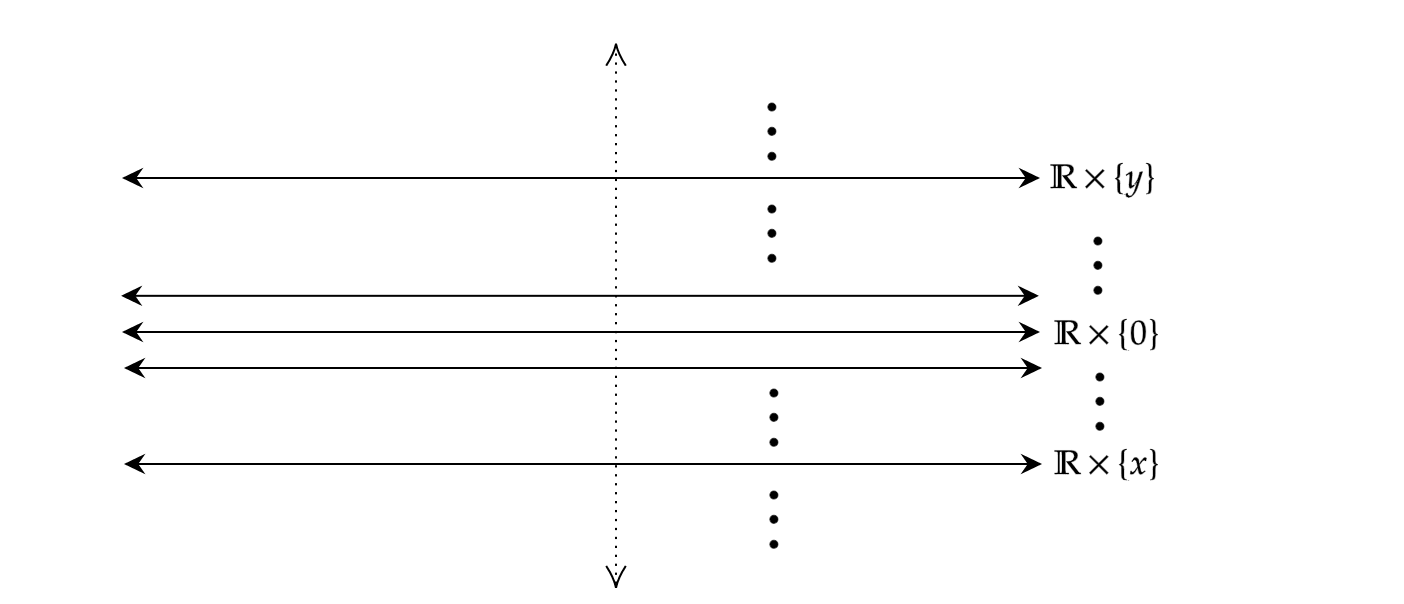
\includegraphics[width = 1.1\textwidth]{diag-4.png}
    \caption{A pictorial view of the space}
\end{figure}
\end{block}
\end{frame}
\begin{frame}{Thank you!}
    Any questions or suggestions?
    
    \alert{P.S. An apology:} \\
    I tried to reduce textual content, as I had remarked in the previous presentation however mathematical rigour does require a good amount of text, if ambiguity has to be left out, for the reader.
\end{frame}



%\section{Sreehari Bodas}

%\section{Atharva Pangarkar}


%\section{Nishtha Sinha}

%\section{Amisha Jangra}




%---------------------------------------------------------
%Example of the \pause comman
%---------------------------------------------------------



%---------------------------------------------------------


\end{document}